% ============================================================================
% WORKSHEET - Section 1.5: Graphing Proportional Relationships
% CCSS 7.RP.A.2d
% ============================================================================
\section{Graphing Proportional Relationships}
\setcounter{wsNumber}{0}

\begin{worksheetSkills}
\begin{itemize}
    \item Plot proportional relationships on coordinate planes
    \item Interpret $(0, 0)$ and $(1, r)$ on proportional graphs
    \item Connect steepness to the unit rate in $y = kx$
\end{itemize}
\end{worksheetSkills}

\worksheetHeader{Plot the Rate}

\begin{drawSolve}{Graph the Juice Stand Data}

The table shows cups of lemonade sold after each hour.

\bigskip
\begin{center}
\begin{tabular}{|C{3cm}|C{3cm}|}
\hline
\textbf{Hours} & \textbf{Cups Sold} \\
\hline
$0$ & $0$ \\
$1$ & $18$ \\
$2$ & $36$ \\
$3$ & $54$ \\
$4$ & $72$ \\
\hline
\end{tabular}
\end{center}

\bigskip
Plot the points and draw the line that fits the data.

\begin{center}
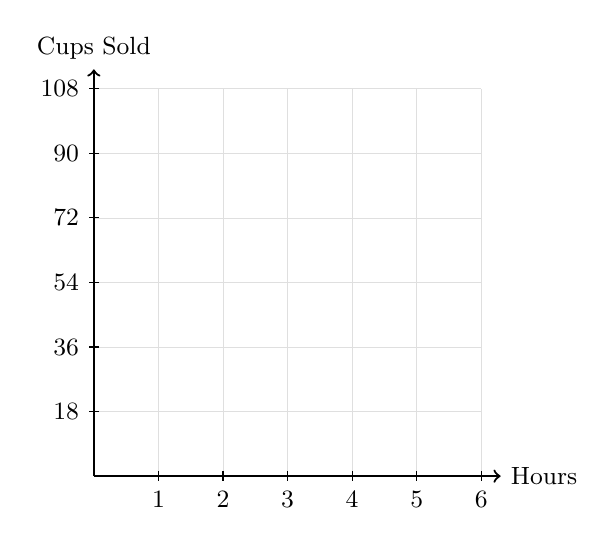
\begin{tikzpicture}[scale=0.82]
\draw[step=1, gray!25, very thin] (0,0) grid (6,6);
\draw[thick, ->] (0,0) -- (6.3,0) node[right]{\small Hours};
\draw[thick, ->] (0,0) -- (0,6.3) node[above]{\small Cups Sold};
\foreach \x in {1,...,6} \draw (\x,0.08) -- (\x,-0.08) node[below]{\small \x};
\foreach \y/\lab in {1/18,2/36,3/54,4/72,5/90,6/108} \draw (0.08,\y) -- (-0.08,\y) node[left]{\small \lab};
\end{tikzpicture}
\end{center}

What is the unit rate? \answerBlank[4cm]

\bigskip

What equation matches this graph? \answerBlank[4cm]
\end{drawSolve}
\worksheetAnswer{The plotted points are $(0, 0)$, $(1, 18)$, $(2, 36)$, $(3, 54)$, and $(4, 72)$. They lie on a straight line through the origin. The unit rate is $18$ cups per hour because the point $(1, 18)$ shows the amount after one hour. The equation is $y = 18x$, where $x$ is hours and $y$ is cups sold.}

\worksheetHeader{Which Graph Tells the Story?}

\begin{matchIt}{Match the Situation to the Graph Clue}

\matchRow{A line through $(0, 0)$ and $(1, 5)$}{Unit rate is $5$}
\matchRow{A line through $(0, 0)$ and $(1, 12)$}{Steeper graph with larger proportional constant}
\matchRow{A line through $(0, 4)$ and $(2, 10)$}{Not proportional because it does not start at zero}
\matchRow{A graph with points $(0, 0)$, $(2, 14)$, $(4, 28)$}{Equation is $y = 7x$}
\matchRow{Two lines through the origin, one with unit rates $3$ and $8$}{The line with unit rate $8$ is steeper}
\end{matchIt}
\worksheetAnswer{A line through $(0, 0)$ and $(1, 5)$ matches ``Unit rate is $5$'' because the $y$-value at $x = 1$ is the unit rate. A line through $(0, 0)$ and $(1, 12)$ matches ``Steeper graph with larger proportional constant'' because $12 > 5$. A line through $(0, 4)$ and $(2, 10)$ matches ``Not proportional because it does not start at zero'' since the origin is missing. The graph with $(0, 0)$, $(2, 14)$, and $(4, 28)$ matches ``Equation is $y = 7x$'' because $14 \div 2 = 7$ and $28 \div 4 = 7$. Two lines with unit rates $3$ and $8$ match ``The line with unit rate $8$ is steeper'' because a bigger constant means more rise for each step to the right.}

\worksheetHeader{Graph Mistake Hunt}

\begin{errorDetective}{Correct the Graph Reasoning}

Student A says: ``The point $(1, 24)$ means the graph has unit rate $24$ pages per hour.''
\errorWork{The graph also includes $(0, 0)$, $(2, 48)$, and $(3, 72)$. Student A says the equation is $y = 24 + x$.}
Correct or wrong? \answerBlank[2cm] \quad Correct equation: \answerBlank[5cm]

\bigskip

Student B says: ``A graph through $(2, 10)$ and $(4, 20)$ is not proportional because $(1, 5)$ is missing.''
\errorWork{Only graphs that show the point $(1, r)$ are proportional.}
Correct or wrong? \answerBlank[2cm] \quad Why? \answerBlank[6cm]

\bigskip

Student C says: ``A line through $(0, 3)$ and $(2, 9)$ has unit rate $3$ because the graph rises by $6$ in $2$ steps.''
\errorWork{Since $9 - 3 = 6$ and $2 - 0 = 2$, the rate is $3$, so the relationship is proportional.}
Correct or wrong? \answerBlank[2cm] \quad Why? \answerBlank[6cm]
\end{errorDetective}
\worksheetAnswer{All three statements are wrong. (1)~Student A correctly noticed that $(1, 24)$ gives a unit rate of $24$, but the equation for a proportional relationship must be $y = kx$, so the correct equation is $y = 24x$, not $y = 24 + x$. (2)~Student B is wrong because the graph can still be proportional even if the point $(1, r)$ is not explicitly shown. The points $(2, 10)$ and $(4, 20)$ both give $k = 5$, so the graph would include $(1, 5)$ and $(0, 0)$. (3)~Student C found a slope of $3$, but the graph is not proportional because it starts at $(0, 3)$ instead of $(0, 0)$. A nonzero intercept means there is a starting amount, so the relationship is not proportional.}

\worksheetHeader{Compare Two Lines}

\begin{mathScenario}{Which Delivery Team Is Faster?}

Two delivery teams travel at constant rates.

\bigskip
\scenarioItem{Team Red}{Graph passes through $(1, 14)$ and $(3, 42)$}
\scenarioItem{Team Blue}{Graph passes through $(1, 18)$ and $(2, 36)$}

\bigskip

What is Team Red's unit rate? \answerBlank[4cm]

\bigskip

What is Team Blue's unit rate? \answerBlank[4cm]

\bigskip

Which graph would be steeper, and what does that mean in context? \answerBlank[8cm]
\end{mathScenario}
\worksheetAnswer{(1)~Team Red's unit rate is $14$ because $42 \div 3 = 14$ and the point $(1, 14)$ shows the same value. (2)~Team Blue's unit rate is $18$ because $36 \div 2 = 18$. (3)~Team Blue's graph is steeper because its proportional constant is larger: $18 > 14$. In context, that means Team Blue travels farther in the same amount of time.}

\worksheetHeader{Explain $(1, r)$ and Steepness}

\begin{explainIt}{What Do Special Points Tell You?}

Explain why the point $(1, r)$ is so useful when looking at a proportional graph.

\writeLines{5}

\bigskip

A friend says, ``The steeper line always means the graph starts higher.'' Explain the difference between starting higher and having a greater unit rate.

\writeLines{6}
\end{explainIt}
\worksheetAnswer{(1)~The point $(1, r)$ is useful because when the input is $1$, the output is exactly the unit rate. That lets you read the constant of proportionality directly from the graph without doing much extra work. If a line passes through $(1, 8)$, then the rule is $y = 8x$. (2)~Starting higher means the line crosses the $y$-axis above zero, which shows a starting amount and usually means the relationship is not proportional. A greater unit rate means the graph rises more for each step to the right while still passing through the origin. So steepness is about the constant of proportionality, not about a nonzero start.}

\worksheetDone